%----------------------------------------------------%
% --------- Brief Descriptive Statistics ---------%
%----------------------------------------------------%

\section{Brief Descriptive Statistics}
\label{sec:descriptive_statistics}
The review identified \samplesize articles published between \samplestart and \sampleend. Scientific output in the field has accelerated in recent years, with the majority of papers published after 2020, peaking in 2024 with \articlesthisyear publications, illustrated in Figure \ref{fig:scientific_productivity}. Thus, it is possible that the field has advanced significantly over the last years, underscoring the need for a comprehensive literature review.

\begin{figure}[H]
    \centering
    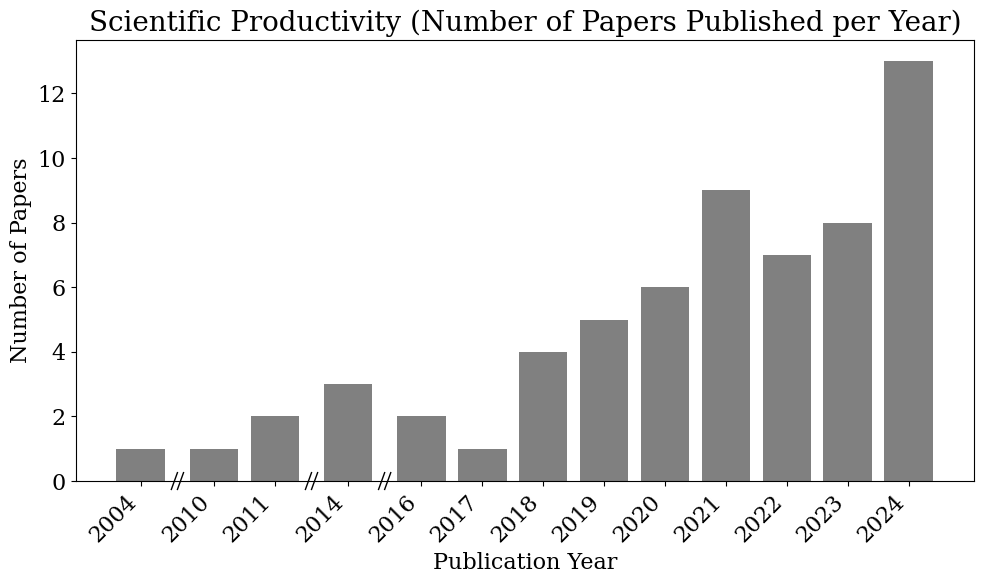
\includegraphics[width=1\linewidth]{Images/scientific_productivity.png}
    \caption[Annual distribution of papers published]{Annual distribution of papers in the field published included in the sample, illustrating the recent increase in publications.}
    \label{fig:scientific_productivity}
\end{figure}

The majority of research originates from China, South-Korea and the US, with 16, 8 and 8 papers contributed by authors from these countries respectively, see Figure \ref{fig:author_country_origin_per_paper}. Each country is counted only once per paper, regardless of the number of contributing authors from that country.  

\begin{figure}[H]
    \centering
    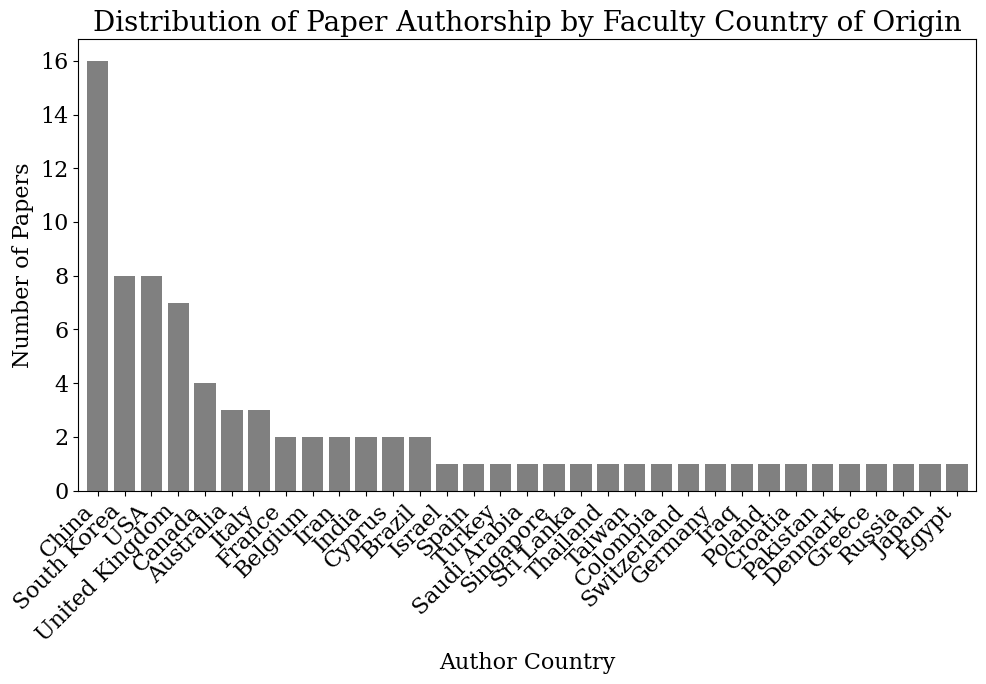
\includegraphics[width=1\linewidth]{Images/author_country_origin_per_paper.png}
    \caption[Number of papers by authors’ faculty country of origin]{Number of papers by authors' faculty country of origin, with each country counted once per article to reflect international collaboration.}
    \label{fig:author_country_origin_per_paper}
\end{figure}

Notably, significant contributions to the field are made by authors from computer science and technical faculties, while only 16\% of authors have a background from financial, business or economics faculties, illustrated in Figure \ref{fig:author_faculty_origin}. To capture the full scope of expertise, all authors are counted individually. 

\begin{figure}[H]
    \centering
    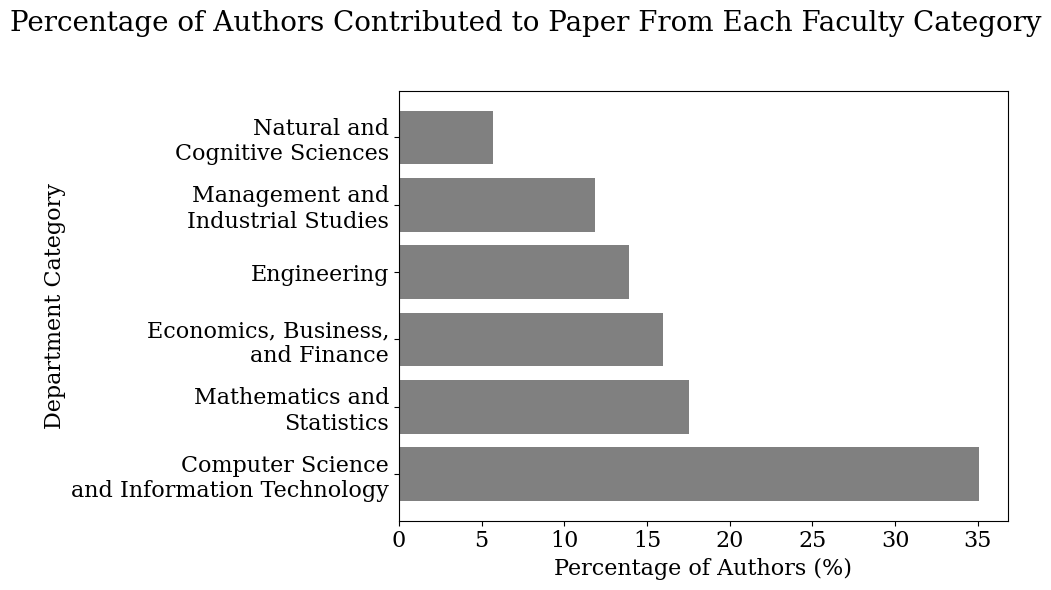
\includegraphics[width=1\linewidth]{Images/author_faculty_origin.png}
    \caption[Percentage distribution of contributing authors by academic faculty category]{Percentage distribution of authors by academic faculty category.}
    \label{fig:author_faculty_origin}
\end{figure}

In terms of journal origins, the majority of the papers in the sample were published in engineering, technical, computer science, and artificial intelligence journals or others. There are only a minor representation in finance and economics journals (15 out of \samplesize papers). Figure \ref{fig:num_papers_per_journal_category} shows the distribution of publications across journal categories. This distribution could suggest a potential gap in domain-specific financial research, indicating an opportunity for increased financial focused journal contributions. The categorization of journals is detailed in Appendix \ref{appendix:journal_category_mapping}. 

\begin{figure}[H]
    \centering
    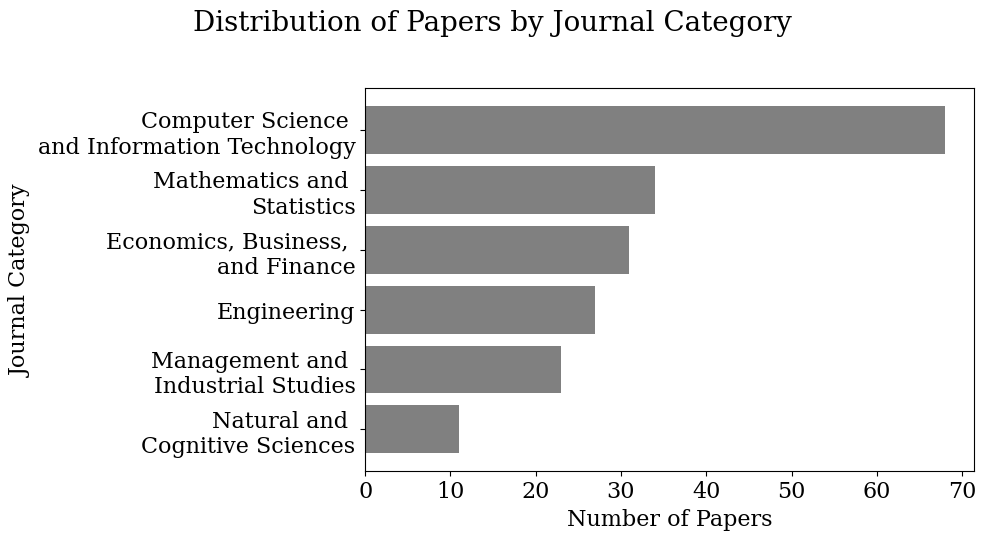
\includegraphics[width=1\linewidth]{Images/num_papers_per_journal_category.png}
    \caption[Number of papers by journal category]{Distribution of sample papers by journal category.}
    \label{fig:num_papers_per_journal_category}
\end{figure}
Only 11 of \samplesize papers disclose the code for the proposed models, as Figure \ref{fig:code_disclosure} illustrates. This lack of disclosure can make reproducibility impossible, as the models are often too complex to enable reproduction based only on article descriptions. Additionally, it makes it more difficult for future researchers to build upon existing research.
\begin{figure}[H]
    \centering
    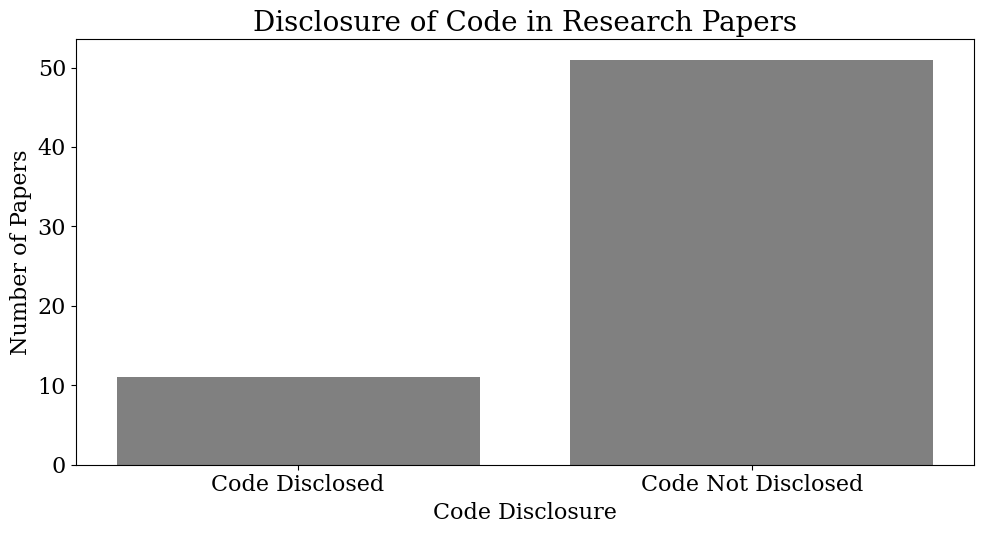
\includegraphics[width=1\linewidth]{Images/code_disclosure.png}
    \caption[Disclosure of model code in research papers]{Disclosure of code in research papers.}
    \label{fig:code_disclosure}
\end{figure}

Figure \ref{fig:treemap_asset_by_market} illustrates the specific financial assets and markets that are forecasted in the studies. The majority of papers focus on equities, primarily stock and stock indices, but a notable number of papers also address currencies and derivatives. Each individual asset predicted in every paper is counted once.   
\begin{figure*}[h]
    \centering
    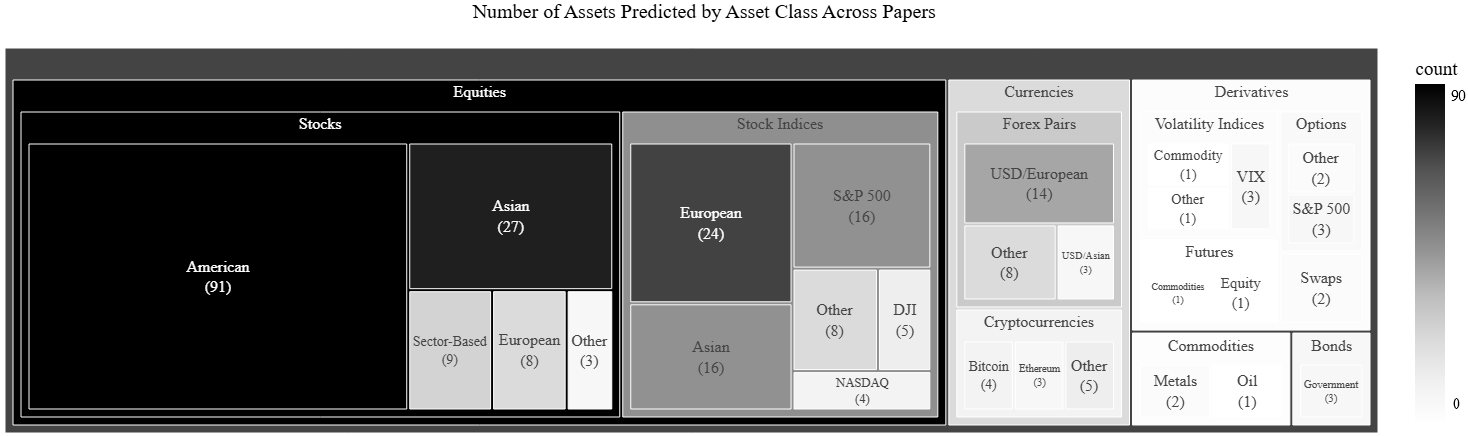
\includegraphics[width=1\linewidth]{Images/treemap_asset_by_market.png}
    \caption[Distribution of financial markets and assets forecasted in the sample]{Distribution of financial markets and assets targeted by the predictive models in the sample papers. \tablefootnote{Sector-Based stocks refer to Select Sector Portfolios like XLB, XLY, etc.}}
    \label{fig:treemap_asset_by_market}
\end{figure*}




%The papers in the samples explores different predictive objectives within the financial domain. As shown in Figure \ref{fig:what_is_predicted}, most papers forecast asset prices, classifications or uncertainty quantification of asset prices. [CHANGE GRAPH AFTER NEW MAPPING]
%\begin{figure}[H]
%    \centering
%    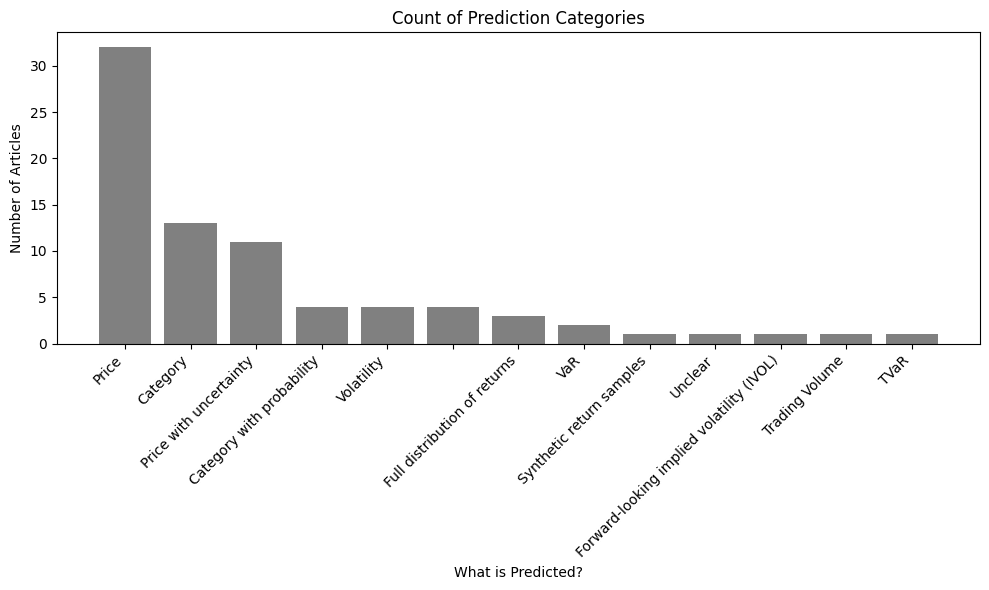
\includegraphics[width=1\linewidth]{Images/what_is_predicted.png}
%    \caption{Distribution of predictive objectives in the sample papers.}
%    \label{fig:what_is_predicted}
%\end{figure}